\section{Expression analysis advanced}
\subsection{Estimating gene expression}
For this practical we need a RNA-seq alignments we previously made in the basic expression analysis: ``\textit{... miR-23b.bam}''.
If you did not do that practical, you can find it in the supplementary material: \\
\datalibrarydirrnaseqadvanced $\rightarrow$ \textit{miR-23b.bam (clean)}\\
Ensure that the file is annotated at reference genome hg19. To estimate expression in RNA-Seq, we can count the number of reads that are aligned to each gene from the list of candidate genes. Therefore you also need to import:\\
\datalibrarydirrnaseqadvanced $\rightarrow$ ucsc\_refseq.gtf\\
This list is provided as a GTF/GFF file.
There are a variety of tools available for counting reads.
FeatureCounts is one of the faster tools and it works directly using BAM files. If you search for:\\
``\textit{\underline{featureCounts} Measure gene expression in RNA-Seq experiments from SAM or BAM files.}''\\
in the Tools menu, you can find the wrapper by the name:\\
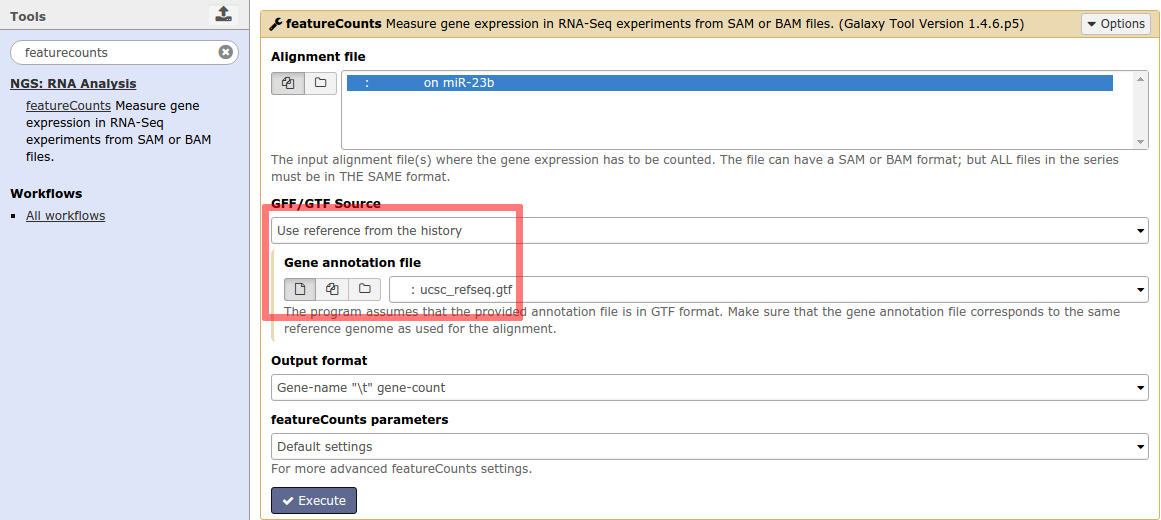
\includegraphics[width=\textwidth]{figures/expression_01.png}\\
Before we proceed, we would like to know whether the analysis has been performed correctly. Therefore we take a look at featureCounts’ output-summary file ``\textit{featureCounts on \ldots}'':
\begin{itemize}
	\item How many reads are \textit{Assigned}?
	\item How many reads are \textit{UnAssigned (sum of all)}?
\end{itemize}
Flagstat told us the alignment has 18258 or 19493 reads in total (different versions).
Please confirm whether this matches with the total number of reads in the featureCounts summary file.

If we want to look at a particular gene, we may want to truncate the large table and only show the row with the gene of interest.
To filter a tabular file we proceed with the following Galaxy tool: 
\textit{\underline{Filter} data on any column using simple expressions}:\\
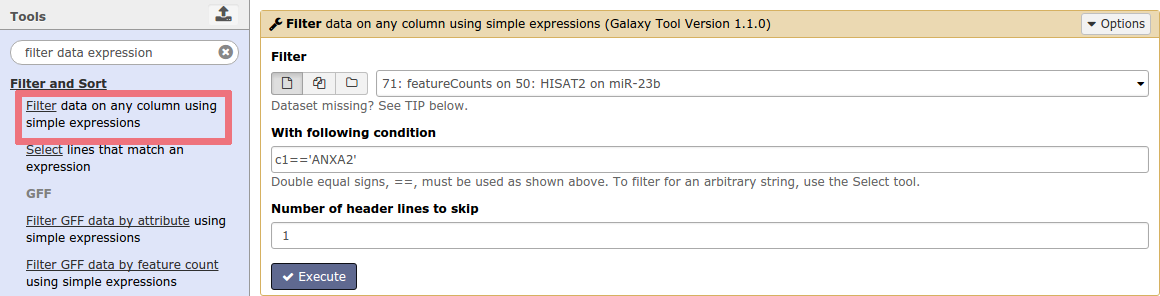
\includegraphics[width=\textwidth]{figures/expression_02.png}\\
\begin{itemize}
	\item How many reads are aligned to DRAM1?
	\item Which gene has the highest read count (tip: use \textit{sort})?
\end{itemize}

\subsection{Expression analysis: Low sequencing depth}
In the previous exercise we found which gene had the highest read count, but what does it mean if this gene has a high read count all samples?
To say something about expression levels, we would like to say it in a context relative to other samples.
Therefore, we need normalization and apply statistical testing.
A popular R package that allows to do this is EdgeR, which in galaxy fits perfectly with featureCounts.

In the following analyses you will determine the differentially expressed genes in the MCF-7-cell line between samples that have been treated with the hormone $\beta$-estradiol (E2) and those that were left as control \citep{mcf7}.
The data was originally used to benchmark the statistical power of adding replicates and does not reflect a certain disease state.
In this exercise we will reproduce a part of their experiment to highlight the importance of replicates.
However, it is a 2-class problem and has a similar setup as often used in cancer analysis.
Before we proceed, please read the abstract of the following article:
\url{http://dx.doi.org/10.1093/bioinformatics/btt688}\\
Tip: Look up from what tissue the MCF-7 cell line originates.\\
\\
For this practical we made the read count tables from featureCounts already available.
We will analyse the samples with a sequencing depth of $\sim$30M (full), 10M and 5M, for each replicate.
Each analysis in this assignment will be to determine the number of differentially expressed (DE) genes and add this number to Table \ref{tab:dge_ad_01}.
\begin{table}[]
\centering
\caption{results of DGE analysis}
\label{tab:dge_ad_01}
\begin{tabular}{ | l | l | r | }
\hline
Replicates & Seq. Depth & Significant DE genes \\
\hline
0          & 0          & 0\quad\quad \\
7rep\_5M   & 5,000,000  & \verb|.......| ? \\
7rep\_10M  & 10,000,000 & \verb|.......| ? \\
7rep\_30M  & 30,000,000 & \verb|.......| ? \\
5rep\_30M  & 30,000,000 & \verb|.......| ? \\
\hline
\end{tabular}
\end{table}
Import the following files from data library \textit{\datalibrarydirrnaseqadvanced}:
\begin{itemize}
	\item[] \verb|GSE51403_expression_matrix_5M_coverage.txt|
	\item[] \verb|GSE51403_expression_matrix_10M_coverage.txt|
	\item[] \verb|GSE51403_design_matrix_subsampled.txt|
\end{itemize}
The design matrix provides the mapping from the RNA-seq read counts per sample to the phenotype class each is associated with.
Please take a look at file \verb|GSE51403_design_matrix_subsampled.txt|
\begin{itemize}
	\item Given that the first column lists the names of the samples and the second column the samples' corresponding condition, how many conditions does the experiment have?
\end{itemize}
\subsubsection{Subsampled datasets: 5M, 7+7}
For our experiment we have a 2-classes setup: a class treated with estradiol is called ``E2'', and the other is called ``Control''.
Take one more look at the design matrix and see if you can find samples that belong to these classes.
Go over the following steps to find the differentially expressed genes between ``E2'' and ``Control'' using 7 replicates per condition and 5 million reads per sample.

Note: although the design matrix contains a class description for all samples, also with 10M, 25M reads and class ``Unknown'', while the expression matrix contains only those for 5M reads, the edgeR wrapper will link the samples based on their sample name and proceed with those.
\begin{itemize}
	\item [$\square$] Load ``\textit{\underline{edgeR: Differential Gene(Expression) Analysis} RNA-Seq gene expression analysis using edgeR (R package)}
	\item [$\square$] Choose \textbf{Analysis type}: \textit{Multigroup test and/or complex designs with e.g. blocking}
	\item [$\square$] Choose \textbf{Expression (read count) matrix}: {\scriptsize \verb|GSE51403_expression_matrix_5M_coverage.txt|}
	\item [$\square$] Choose \textbf{Design matrix}: \verb|GSE51403_design_matrix_subsampled.txt|
	\item [$\square$] Define contrast: this is the more complicated part of the wrapper. It is effectively defining the hypothesis we want to test. This is done via a mathematical formulation in a format described by a well known R package \textit{limma}. For two class problems it is very simple: \textit{classNormal-classTreated} which in our case is: \textbf{Control-E2} (case sensitive!)
	\item [$\square$] Set \textbf{Report differentially expressed genes} to \textit{Only significant (defined by FDR cutoff)} and ensure the cutoff is set to \verb|0.01|.
	\item [$\square$] Don't select additional output files and leave the rest default.
	\item [$\square$] Press [Execute]
\end{itemize}
It is always important to check whether we did not make obvious mistakes.
Take a look at the file ``\textit{edgeR DGE on \ldots: GSE51403\_design\_matrix.txt differentially expressed genes}''. If everything is correct, the gene \verb|GREB1| is located in the top of the file. Please check its corresponding gene cards page:\\
\url{http://www.genecards.org/cgi-bin/carddisp.pl?gene=GREB1}\\

\begin{itemize}
	\item Can you find on the gene cards page a regulatory factor of the gene that relates
to the E2 treatment?
	\begin{itemize}
		\item Hint: what was E2 again?
	\end{itemize}
	\item Can you find on the gene cards page an association with MCF-7 cells?
	\begin{itemize}
		\item Hint: what is MCF-7 for type of cell line?
	\end{itemize}
\end{itemize}
The answers to the questions should confirm that what we found with the expression analysis is in agreement with the biology behind it.
If we go back to the output file, each line represents one gene, indicated by the gene symbol in the 2nd column.
Because the table is ordered by FDR, the first column is the original position in the GTF file.
The P-value, 6th column, is a probability that represents the chance to find the read counts that belong to the gene, given that they are from the same condition.
The FDR is a multiple testing correction of the P-value and is usually used instead of the P-value. The lower this value, the less likely it is that the observed values are derived from the same condition. Thus, differentially expressed genes will have a low FDR and P-value for determining significance.
To distinguish between differences considered to be caused by chance or by the different conditions, we make use of a cut-off, commonly set to $\leq 0.01$ or $\leq 0.05$.

In edgeR we already selected to only return those genes with a FDR $\leq 0.01$.
Hence, the number of lines in the history, minus 1 (header line) should give us the number of differentially expressed genes.
\begin{itemize}
	\item How many genes are significant differentially expressed between Control and E2? 
	\begin{itemize}
		\item[$\square$] Please fill this in into Table \ref{tab:dge_ad_01}.
	\end{itemize}
\end{itemize}

\subsubsection{Subsampled datasets: 10M, 7+7}
In the previous analysis, the original FASTQ files used to generate the read count table, contained a total of 5.000.000 reads per sample.
For the next analysis we will make use of twice the amount of raw data to see how the number of differentially expressed genes change: 10M reads per sample, 7 samples per condition.

\begin{itemize}
	\item [$\square$] Re-run the previous job with the rerun icon
	\item [$\square$] Replace \textbf{Expression (read count) matrix}: \textit{GSE51403\_expression\_matrix\_\underline{5M}\_coverage.txt} with \textit{GSE51403\_expression\_matrix\_\underline{10M}\_coverage.txt}
	\item How many genes are significant differentially expressed between Control and E2? Is this more or less than when we used 5M reads?
	\begin{itemize}
		\item[$\square$] Please fill this in into Table \ref{tab:dge_ad_01}
	\end{itemize}
\end{itemize}

\subsubsection{Subsampled datasets: 30M, 7+7}
In the previous analyses, the FASTQ files contained a total of 5.000.000 or 10.000.000 reads per sample. The full data set contains more or less 30.000.000 raw reads per sample. Import the following files from shared data:

\begin{itemize}
	\item[] \verb|GSE51403_expression_matrix_full.txt|
	\item[] \verb|GSE51403_expression_matrix_full_5x5.txt|
	\item[] \verb|GSE51403_design_matrix_full_depth.txt|
\end{itemize}
Proceed with the following steps:
\begin{itemize}
	\item [$\square$] Re-run the previous job with the rerun icon
	\item [$\square$] Replace \textbf{Expression (read count) matrix}: \textit{GSE51403\_expression\_matrix\_\underline{10M}\_coverage.txt} with \textit{GSE51403\_expression\_matrix\_\underline{full}.txt}
	\item [$\square$] Replace \textbf{Design matrix}: \textit{GSE51403\_design\_matrix\_\underline{subsampled}.txt} \\
	 with \textit{GSE51403\_design\_matrix\_\underline{full\_depth}.txt}
	\item How many genes are significant differentially expressed between Control and E2?
	\begin{itemize}
		\item[$\square$] Please fill this in into Table \ref{tab:dge_ad_01}.
	\end{itemize}
\end{itemize}

\subsubsection{Subsampled datasets: 30M, 5+5}
We did three tests with 7+7 replicates and different sequencing depths.
To see what the effects are of sample replication, we should run the same analysis but use a different number of replicates.
To modify expression matrices within Galaxy (both concatenating and removal) we can make use of the tool ``\textit{\underline{edgeR: Concatenate Expression Matrices} Create a full expression matrix}''. We have used all our replicates in the previous analyses and so we can reduce the number of replicates to 5+5 by simply picking a subset:\\
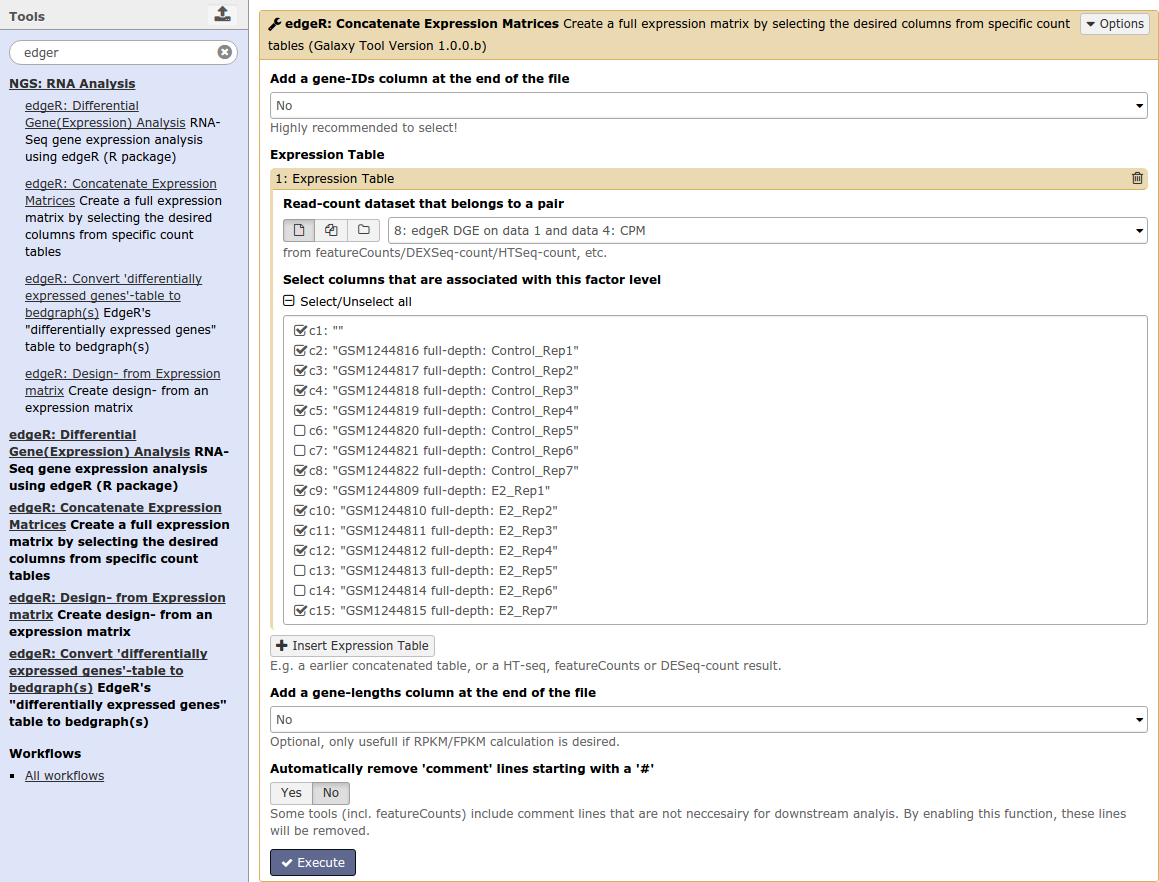
\includegraphics[width=\textwidth]{figures/expression_03.png}\\
This will create a truncated version of the expression matrix, only including the desired 5+5 replicates.
\begin{itemize}
	\item [$\square$] For convenience, rename the new expression matrix to:\\ \verb|GSE51403_expression_matrix_full_5+5_replicates.txt|
	\item [$\square$] Re-run the previous edgeR DGE job with the rerun icon, make sure that the design matrix is \textit{GSE51403\_design\_matrix\_\underline{subsampled}.txt}
	\item [$\square$] Replace \textbf{Expression (read count) matrix}: \textit{GSE51403\_expression\_matrix\_\underline{full}.txt}\\ with \textit{GSE51403\_expression\_matrix\_\underline{full\_5+5\_replicates}.txt}
	\item [$\square$] \textbf{Enable} the optional output: \textit{MDS-plot (logFC-method)}
	\item [$\square$] Set the \textbf{Output format of images} to: \textit{Portable document format (.pdf)}
	\item How many genes are significant differentially expressed between Control and E2?
	\begin{itemize}
		\item[$\square$] Please fill this in into Table \ref{tab:dge_ad_01}.
	\end{itemize}
\end{itemize}
Take a look at the MDS plot.
If you want to understand all details about MDS you should do some research online because it is a complicated mathematical operation.
For now, what matters is that the distances between the samples in the plot should correspond more or less to the distances between the samples based on the expression of all (22.000) genes.
Hence, samples that are far apart in this plot, differ more in their expression profile, and samples that are close to each other, have a more similar expression profile.
\begin{itemize}
	\item Do you see separation between the samples from E2 and Control?
	\item Could you think of an application where it would be desired to see separation between classes?
	\item Would you expect more or less differentially expressed genes if the experiment was done on individual patient samples instead of cell-line replicates?
\end{itemize}
Can you create a tab delimited file of Table \ref{tab:dge_ad_01}, e.g. in notepad or Excel, and upload it as a `tabular' file within Galaxy?
If you are not able to create the file, you can pick the file from the data library:
\datalibrarydirrnaseqadvanced $\rightarrow$ \textit{table\_01}\\
Try to open the table in Galaxy as Scatterplot (visualization on the history item) and discuss with other people about the impact of removing these 2 replicates on the statistical power:\\
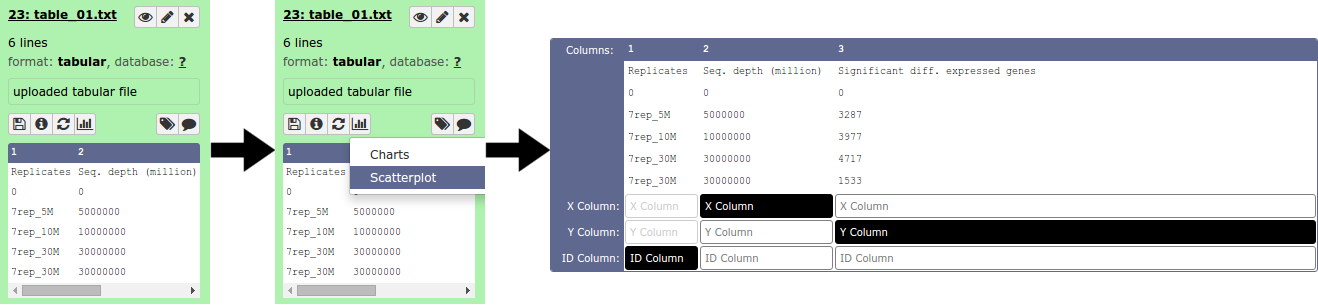
\includegraphics[width=\textwidth]{figures/expression_04.png}\\
\textbf{You are finished!}
\subsection{Bonus question}
In case you can't get enough of it, go to the Shared Data bonus section and answer the following question:
\begin{itemize}
	\item To which classes do the Unknown samples belong? (hint: MDS)
\end{itemize}
